%
% Thesis template conforming to Williams College rules.
% Thanks to Ben Wood '08 and other contributors.
%
\documentclass[twoside]{report}
\usepackage[top=1.0in, bottom=1in, left=1.5in, right=1in, includehead]{geometry}
\pagestyle{headings}
\usepackage{setspace}
%% Special math fonts and symbols
\usepackage{amssymb}
\usepackage{amsfonts}
\usepackage{amsmath}
\usepackage{amsthm}
%% Rotate tables and figures
\usepackage{rotating}
%% Used for TODO items
\usepackage{color}
%% used for code listings.
\usepackage{float}
%% Used to replace LaTeX's ugly emptyset with diameter, which looks nicer.
\usepackage{wasysym}
%% Nicely formatted algorithms.
\usepackage{algorithmicx}
\usepackage[chapter]{algorithm}
\usepackage{algpseudocode}
%% Nicely formatted listings.
\usepackage{listings}
%% More kinds of arrow with stuff
\usepackage{empheq}
\usepackage{multicol}
\usepackage{subfigure}
%%%%%%%%%%%%%%%%%%%%%%%%%%%%%
%% Thesis body %%
%%%%%%%%%%%%%%%%%%%%%%%%%%%%%
\begin{document}
%%%%%%%%%%%%%%%%%%%%%%%%%%%%%
%% Title page %%
%%%%%%%%%%%%%%%%%%%%%%%%%%%%%
\begin{titlepage}
$\;$
\vskip1.5in
\onehalfspacing
\begin{center}
{\LARGE
Title
}
\large
\vskip.25in
by\\
Kurt Gu\\
\vskip.125in
Professor Kelly Shaw, Advisor\\
\singlespacing
\vskip.5in
\small
A thesis submitted in partial fulfillment\\
of the requirements for the\\
Degree of Bachelor of Arts with Honors\\
in Computer Science\\
\vskip.5in
Williams College\\
Williamstown, Massachusetts\\
\vskip.5in
\today
%%\vskip.5in
%%{\Huge \textbf{DRAFT}}
\end{center}
\end{titlepage}
%%%%%%%%%%%%%%%%%%%%%%%%%%%%%
\tableofcontents
\listoffigures
\listoftables
\onehalfspacing
\chapter*{Abstract}
\chapter*{Acknowledgments}
%%%%%%%% Chapters %%%%%%%%%%%%
%% Introduction
\chapter{Introduction}
\section{Motivation}
\section{Summary}

\chapter{Background}
\section{Summary}

\chapter{Methodology}
In this thesis, we will be implementing a small energy-harvesting device using physical hardware, 
on which we will run two software applications and evaluate how our proposed mitigations affect 
their energy efficiency performances. 
This chapter introduces the specific hardware and software components used to build our device, 
the applications that will run on the device, 
and the testing methodology we use to determine the energy efficiency of those applications.

\section{Hardware Tools}
\subsection{System Overview} \label{overview}
Our test device consists of four major parts:
\begin{enumerate}
    \item The microcontroller unit (MCU) connects to all other periphral components, 
          and handles data processing and computation.
    \item The power supply, which itself contains three parts: the supercapacitor that serves 
          as the battery for the device, the supercapacitor manager that uses incoming harvested 
          power to charge the supercapacitor, and finally the energy harvester such as a solar panel. 
          In our case, we use a variable power supply in place of an energy harvester for better 
          consistency and stability between different experiments.
    \item The camera module, which captures image sensory data.
    \item The long range radio, or LoRa, which transmits the data captured and processed by our device 
          to an external and distant receiver.
\end{enumerate}

\begin{figure}[ht]
    \centering
    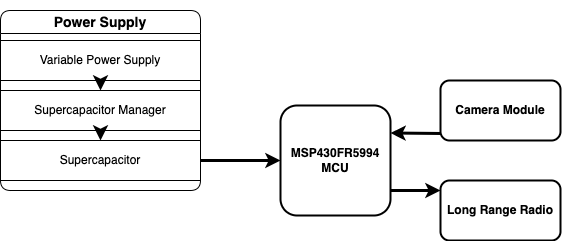
\includegraphics[width=0.8\linewidth]{method/3.1.png}
    \caption{Diagram of component connections.}
    \label{fig:connection}
\end{figure}

Figure \ref{fig:connection} is a diagram of how the components in our device are connected to each other. 

\subsection{Component Selection}
\begin{enumerate}
    \item MCU: For our device, we select the MSP430FR5994 low-power MCU from Texas Instruments (TI). 
    This is an MCU with $8$kB of RAM, $256$kB of nonvolatile memory, and a clock frequency range between 
    $10$kHz to $24$MHz. It also carries an onboard temperature sensor. 
    Specifically, we are using the LaunchPad development kit for this MCU, which comes with headers for 
    the MCU's general purpose IO pins for easy connection to periphrals, and
    includes an onboard debug probe for programming, debugging and energy measurements. 
    The dev kit is also equipped with a microSD card slot, and a small onboard supercapacitor battery.
    \item Power supply: We select the AEMSUCA [tindie source] based on the AEM10941 chip as our 
    supercapacitor manager for its wide compatibility and low cost. For the supercapacitor, we select 
    a 1F, 2.7V capacitor from Kemet[source], which achieves a good balance between capacity and size.
    \item Camera module: We select the low-power HM01B0 camera module, which is capable of capturing images up to 
          $320$x$320$ pixles in size.
    \item Long range radio: We select the RFM95W long range radio transceiver. It has a transmission range of 
          approximately $2$ kilometers or $1.24$ miles, and operates in either the 868 or 915 MHz channel.
\end{enumerate}
\subsubsection{Processor Architecture}
*See fig.3.2*, more detail on the architecture of the specific chip we are using.
\begin{figure}[ht]
    \centering
    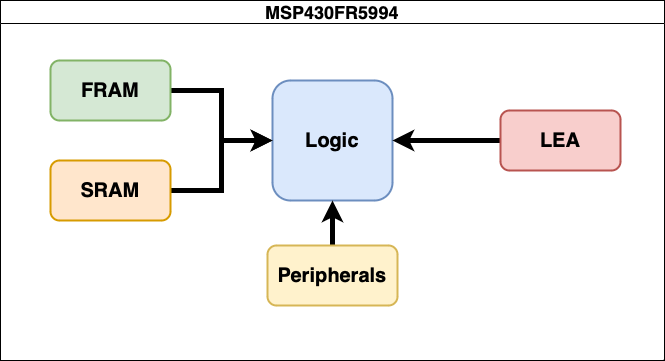
\includegraphics[width=0.8\linewidth]{method/arch.png}
    \caption{Architecture of}
    \label{fig:arch}
\end{figure}

\subsection{Component Power Consumption}
Since the focus of this thesis is optimizing energy efficiency, we should pay attention to hardware power 
consumption. Therefore, in table \ref{tab:power} we include a list of power draws for each of our components. 
Note that the power consumption of the MCU varies under different workloads. It typically increases as the workload becomes more computationally 
intensive, and as the clock frequency increases.

\begin{table}[ht]
\begin{center}
    \begin{tabular}{ |c|c|c| } 
     \hline
     \textbf{Component} & \textbf{State} & \textbf{Power Draw (mW)} \\
     \hline
     MCU & Low Power(10-32 kHz clock, periphals off) & 0.34 \\ 
     \hline
     MCU & Normal(1 MHz clock) & 1.22 \\ 
     \hline
     MCU & High Frequency (24 MHz clock) & 2.2 \\ 
     \hline
     Camera & Standby & $< 0.2$ \\
     \hline
     Camera & Active ($160$x$120$ pixels @ $30$ fps) & $< 1.1$ \\
     \hline
     Camera & Active ($320$x$320$ pixels @ $30$ fps) & $< 2$ \\
     \hline
     Radio & Standby & 6 \\
     \hline
     Radio & Transmit & 66 - 396 \\
     \hline
    \end{tabular}
    \caption{Component power draws [sources]}
\end{center} \label{tab:power}
\end{table}

\begin{figure}[ht]
    \centering
    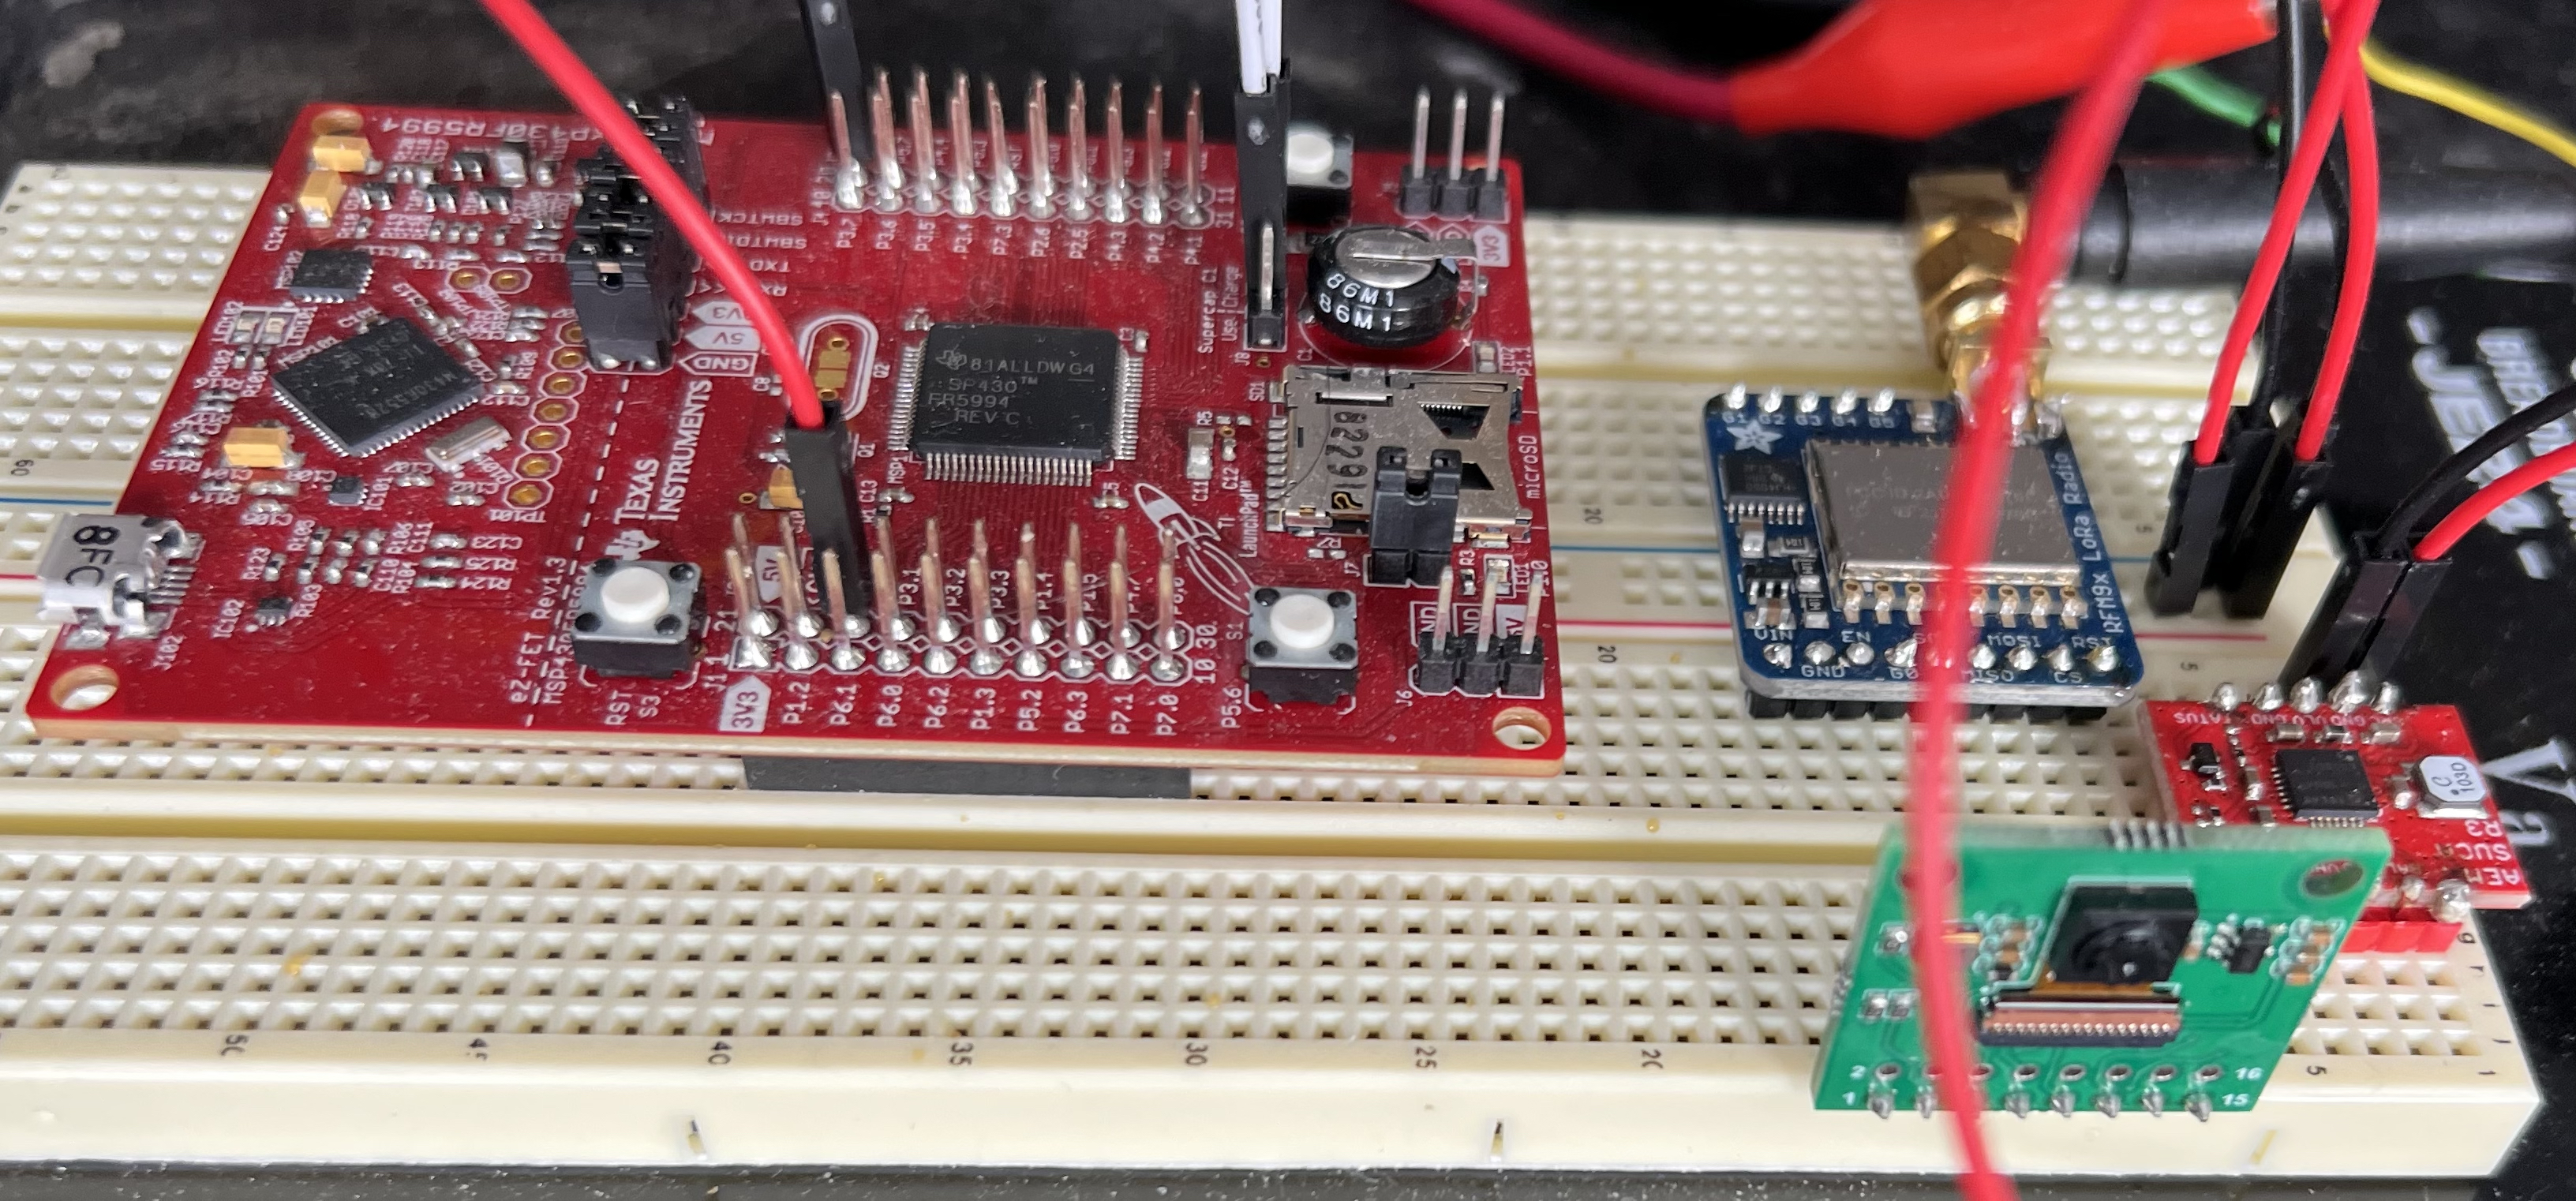
\includegraphics[width=0.8\linewidth]{method/device.jpg}
    \caption{Our test device, with each component labeled.}
    \label{fig:device}
\end{figure}

\section{Software Tools}
In this thesis, we write software to test the performance of our proposed efficiency mitigations. 
The main saftware tasks required to perform the tests are as follows:

\begin{enumerate}
    \item Load data from SD card for local inference, or poll onboard sensor for temperature data.
    \item Process the captured data to determine if it is an event of interest.
    \item Communicate with the long range radio chip to transmit interesting data.
    \item Based on the running task, adjust clock frequency to either save power or boost performance.
    \item Execute all the tasks above according to a user-specified schedule.
\end{enumerate}

In this section, we introduce the software tools used to implement the tasks above.

\subsection{Software Environment}
To program the device, we use TI's own integrated development environment (IDE) called 
Code Composer Studio (CCS) [source]. Source code is written in C, and CCS compiles our C code using MSP-CGT, 
which is TI's code generation tool for compiling device-specific assembly code. CCS then load the compiled code onto 
our device through the onboard debugger via a USB connection. CCS's code editor also provides advice 
on best practices for writing energy efficient C code.

\subsection{External Packages}
Working with embedded MCUs such as the MSP430 series often involve programming directly at the register level, 
which requires writing complex code with low readbility. 
For a quicker and simpler development process, we use a number of external packages developed by TI and 
the open-source community. For example, the MSP430 DriverLib provides methods that alter the MCU's clock frequency, 
so that the programmer no longer needs to manually unlock and modify the registers controlling clock speeds.
Table \ref{tab:packages} provides a list of packages we used during software 
implementation, along with a short description of their usage.

\begin{table}
    \begin{center}
        \begin{tabular}{ |c|c| }
            \hline
            \textbf{Package Name} & \textbf{Description} \\
            \hline
            MSP430 General Library & Standard register and bit definitions for MSP430 microcontrollers, \\
                                   & included with Code Composer Studio. \\
            \hline
            MSP430 DriverLib [cite] & Periphal driver library, allows application development \\
                                    & at an API level, reduces register-level programming.\\
            \hline
            MSP430 DSPLib [cite] & Digital Signal Processing library, contains optimized functions\\
                                 & for vector/matrix operations using fixed-point arithmetics.\\
            \hline
            Lenet-accelerator [cite] & LeNet-5 image classification network,\\
                                     & adpated to the MSP430FR5994 architecture using DSPLib.\\
            \hline
            SDCardLib [cite] & SD card driver library specifically for our development kit, \\
                             & enables writing to and reading from files on an inserted SD card. \\
            \hline
        \end{tabular} 
        \caption{Packages}
        \label{tab:packages}
    \end{center}
\end{table}

\subsection{Development Process}
At a high level, this is how we develop software to perform the tasks listed at the begining of the section:
\begin{enumerate}
    \item To load dataset for local inference, we first load the dataset onto a microSD card, 
    then we interface with the card using TI's SDCardLib library, reading one image at a time and load 
    it onto the device's FRAM.

    \item To poll onboard sensor for temperature data, we use TI's MSP430 DriverLib API to read from 
    the onboard analog-digital converter (ADC) to acqurie the raw reading of the temperature sensor. 
    We then convert this raw data into either Celsius or Farenheit using $2$ reference datapoints: 
    and the following formula: 

    \item To communicate with the long range radio or the camera,
    
    \item The neural network used for local inference was implemented using TI's DSPLib, which contains 
    architecture-specific implementations of matrix and vector operations. The operations implemented 
    in DSPLib are capable of higher performance and efficiency because they take advantage of our particular MCU's low-energy accelerator (LEA), 
    which is a built-in 32-bit hardware accelerator for normally slow and power hungry operations such as 
    matrix multiplication and fast Fourier transforms (FFT). 
    
    \item To adjust clock frequency for power and/or performance reasons, again we use DriverLib 
    to modify the registers on the MCU whose values directly controll its clock frequency.
\end{enumerate}

\section{Software Applications}
In this thesis, we focus on optimizing the energy efficiency for two specific applications: 
inference using a local classification network, and recording environment temperature using an 
onboard sensor. This section introduces general structure of an application running on energy harvesting devices, 
as well as the two specific applications we focus on, while Section \ref{sec:testMethod} 
discusses the efficiency mitigations we propose and test.
\subsection{Application Structure}
\begin{figure}[ht]
    \centering
    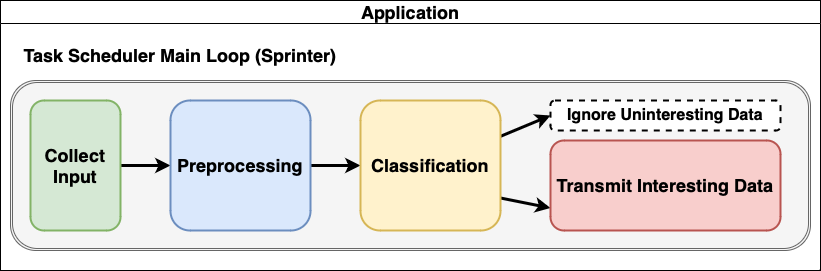
\includegraphics[width=0.9\linewidth]{method/struct.png}
    \caption{Structure of an EH Device Application.}
    \label{fig:struct}
\end{figure}

\subsection{Application: Local Inference}
\subsubsection{Limitations Of Local Inference (Move to Experiments section?)}
As we have discussed previously, running machine learning models locally to classify interesting 
data reduces the frequency of energy intensive data transmissions. 
However, preforming local inference also comes with limitations, 
primarily in terms of model size and performance. Since our MCU has only $8$kB of RAM 
and $256$kB of nonvolatile memory, larger models would not fit in memory. Furthermore, 
since our MCU cannot compute floating point numbers natively, local inference models 
using floating-point weights yield non-ideal performance when run on our device without optimizations.

\subsubsection{LeNet-5 Classification Network}
For this thesis, we use local inference to classify image data as either interesting or uninteresting. 
Specifically, we select the LeNet-5 image classification network[source] as our local inference model. 
First published in 1998 by Yann LeCun et al, LeNet-5 is a relatively small neural network with seven 
total layers, and a reasonable number of weights that can fit onto our device's memory, 
which makes it an ideal candidate for our use. Since LeNet-5 has 
already been adapted to the MSP430 platform using native libraries and fixed-point arithmetics[source], 
it performs well when run on our test device. Furthermore, LeNet-5 has been trained and tested on many 
available datasets, which makes its on-device performance easier to evaluate without compiling our own dataset.

\begin{figure}[ht]
    \centering
    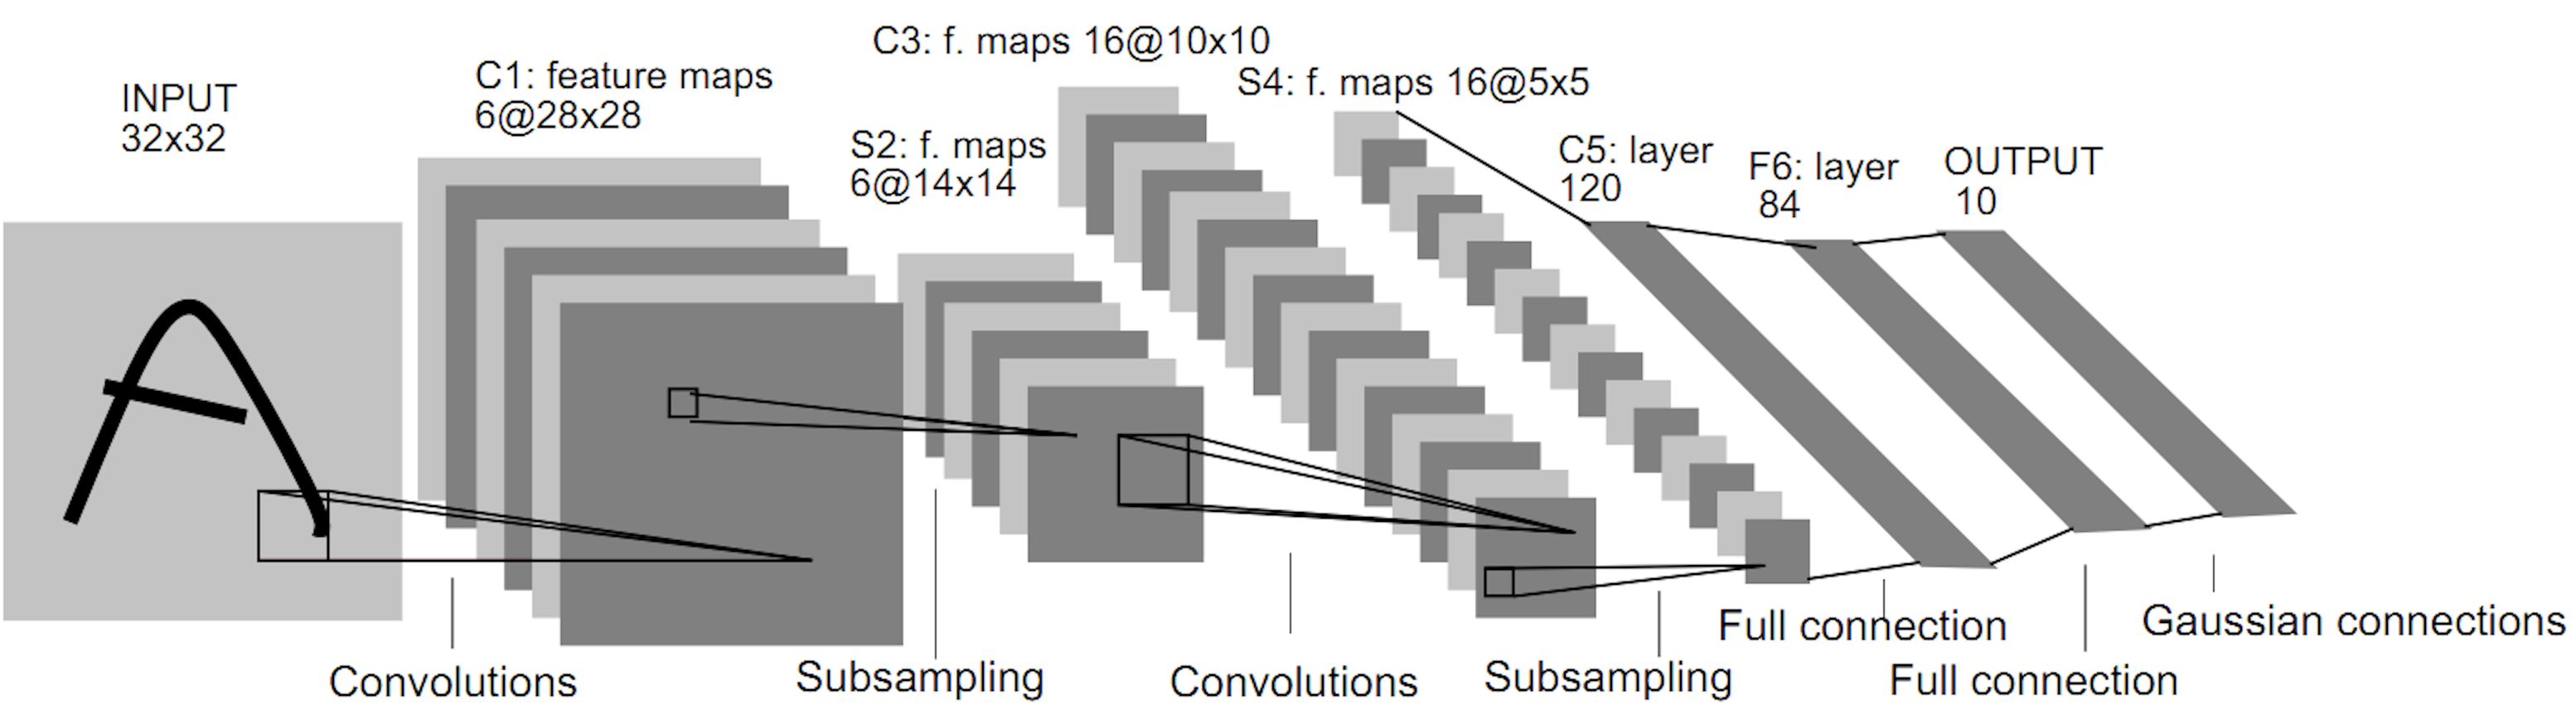
\includegraphics[width=1.0\linewidth]{method/lenet5.png}
    \caption{Structure of LeNet-5.[source]}
    \label{fig:lenet5}
\end{figure}

\subsubsection{Datasets Used For Evaluation}
We use existing datasets to evaluate the performance of our local inference model. Specifically, 
we have identified three datasets that can be used with LeNet:
\begin{enumerate}
    \item MNIST: The Modified National Institute of Standards and Technology (MNIST) database 
          is a collection of handwritten digits($0-9$). Each example in the dataset is a $28\times28$ 
          greyscale image.
    \item Fashion-MNIST: A dataset containing $28\times28$ grayscale images of fashion products 
    from 10 categories, with $7,000$ images in each category.
    \item CIFAR-10: A dataset containing $32\times32$ color images from 10 categories, 
    with $6,000$ images in each category.
\end{enumerate}

\begin{figure}[ht]
    \centering
    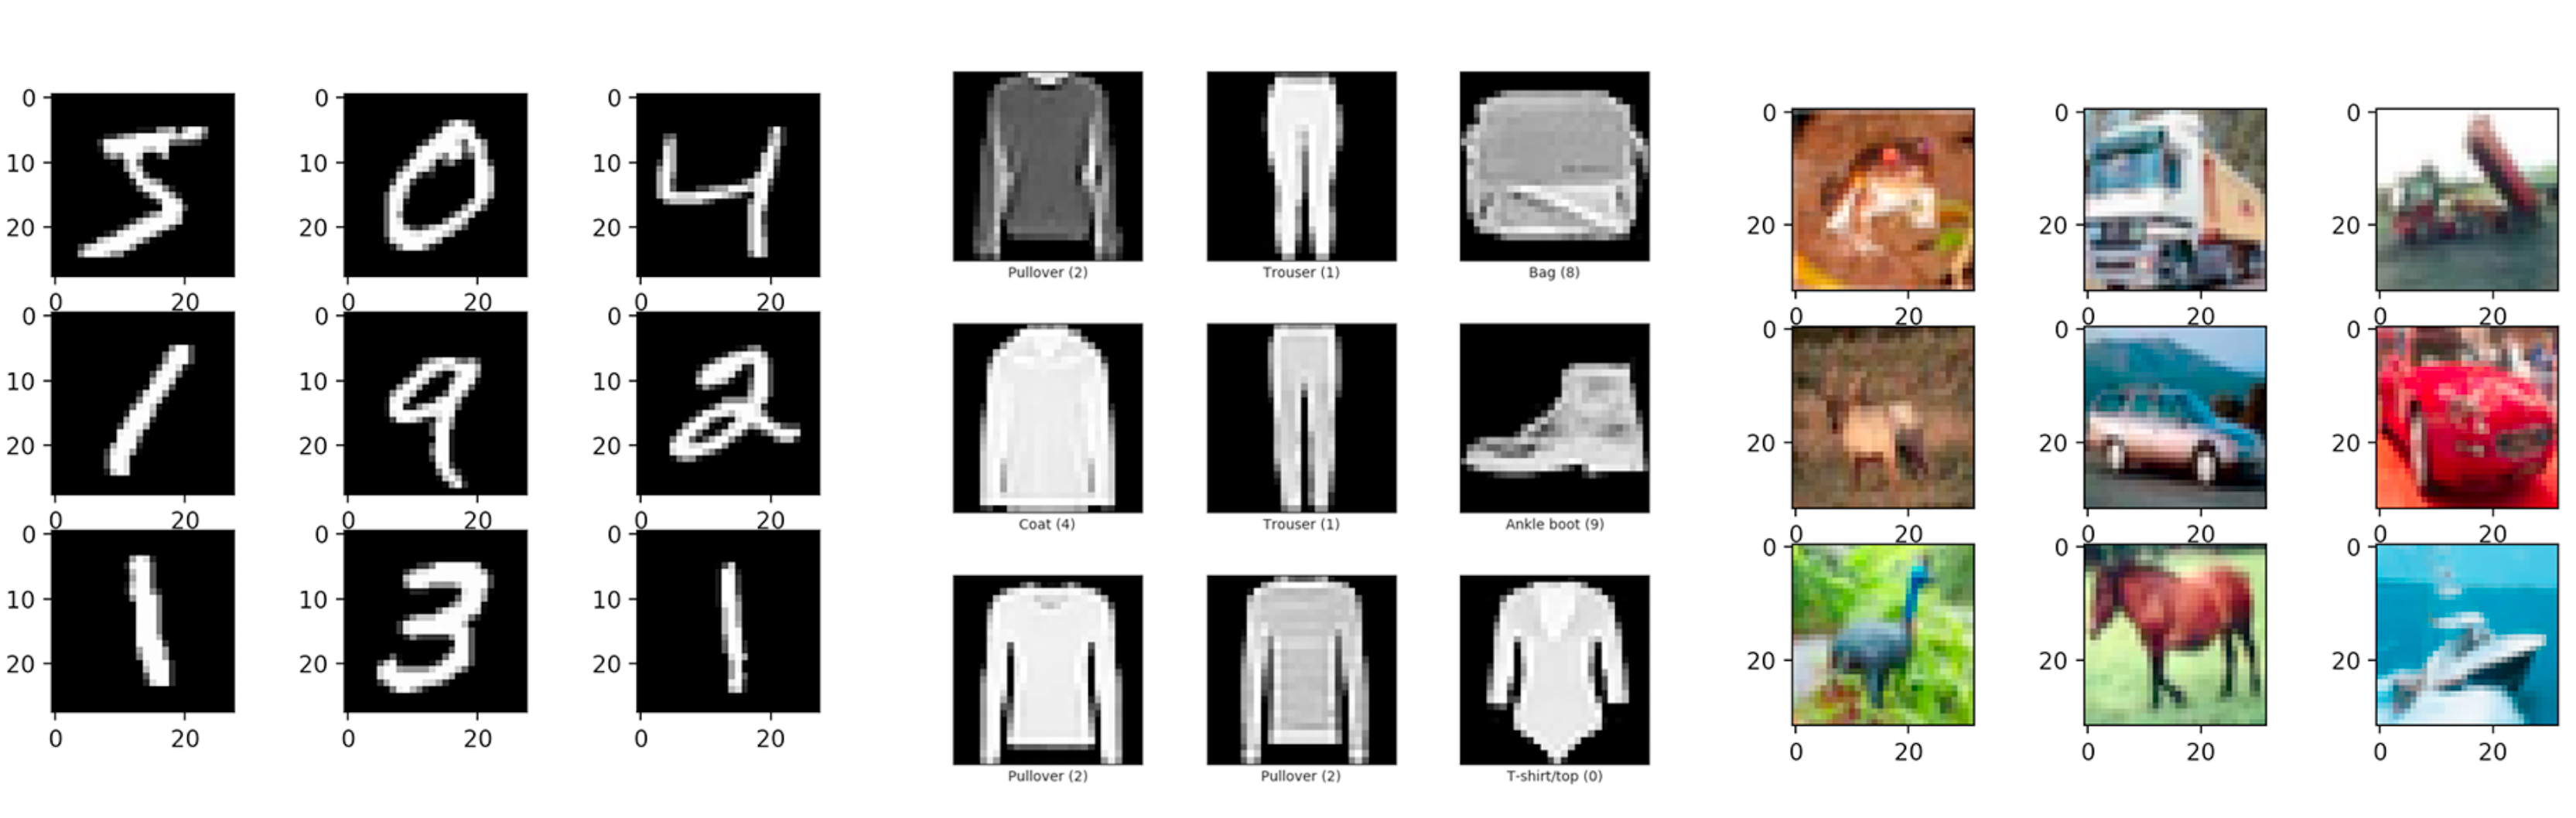
\includegraphics[width=1.0\linewidth]{method/datasets.png}
    \caption{Sample images from datasets used to test ML model performance. \\Left: MNIST, Middle: Fashion-MNIST, Right: CIFAR-10}
    \label{fig:datasets}
\end{figure}

\subsection{Application: Temperature Sensing With Sprinting}
\subsubsection{Data Accquisition}
\subsubsection{Tunable Parameters}
 
\section{Testing Methodology} \label{sec:testMethod}
\subsection{Supplying Power \& Data}
As mentioned in section \ref{overview}, power is supplied to our test device via a variable power supply, 
charging the supercapacitor which then powers the test device. By using a variable power supply, 
we can alter the magnitude of output power to simulate the behavior of a solar panel under 
different lighting conditions. To simulate a cloudy day with low harvested power, we could lower the power 
supply's output current. To simulate a sunny day, we could simply raise the output current.\\\\
For our temperature sensing application, our device generates data in real-time using the on-device sensor. 
However, to evaluate the performance of the local inference application, 
we need to provide our device with test datasets containing hundreds of images, which are too large to fit onto the $256$kB of 
local memory. Therefore, we make use of the onboard SD card slot by loading the test datasets onto 
an microSD card, from which the MCU will then read during testing. The drawback to this approach 
is that the SD card requires around $40$mW of additional power. However, since this power draw is 
near-constant, it can be treated as a bias in our data and can be factored out easily without 
affecting data accuracy.

\subsection{Monitoring Power With Energytrace}
Energytrace is a power monitoring tool integrated in CCS that works with our development kit. 
It monitors the device during operation using the debugger onboard the development kit, 
and provides the programmer with in-depth information about the device's power consumption behavior.\\\\
As an example, Figure \ref{fig:traces} contains two sample outputs by Energytrace. 
The Energytrace++ profiler at the top records energy consumption and runtime information 
about each power mode that our device could be in, and about the program being executed on-device, 
while the basic Energytrace profiler at the bottom records the device's electrical information 
during operation, such as voltage, current, average and max power draw, etc.
\begin{figure}[ht]
    \centering
    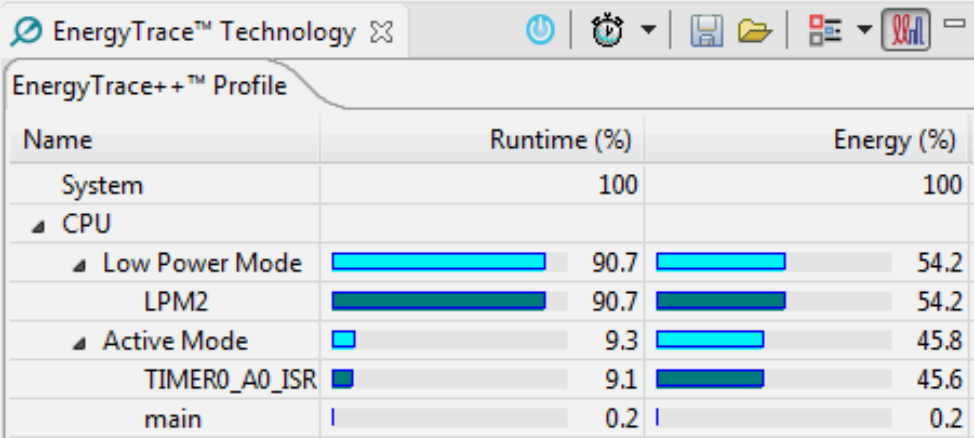
\includegraphics[width=0.8\linewidth]{method/trace2.png}
    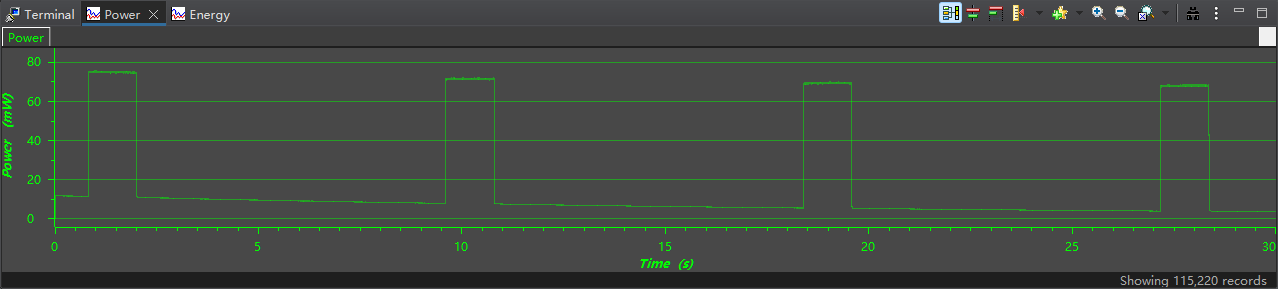
\includegraphics[width=0.8\linewidth]{method/trace.PNG}
    \caption{Example Energytrace outputs.}
    \label{fig:traces}
\end{figure}

\subsection{General Testing Framework (Move to experiments?)}
\subsubsection{Preprocessing Methods}

Recall from chapters that we propose to test different preprocessing methods' effects on energy efficiency. 
In this thesis we will test $2$ preprocessing methods: \textbf{Structural Similarity Index Measure (SSIM)}[source] 
and \textbf{Statistical Analysis}.

Specifically, we proposed \textbf{SSIM} as an alternative to the simple preprocessing method employed in current application
pipelines, where $2$ images are determined different if their pixel values differed by more than a 
heuristically determined threshold. Alternatively, SSIM evaluates the similarity between $2$ images across 
$3$ dimensions: luminance, contrast, and structure. SSIM's formula is as follows (placeholder): 
\[ SSIM: x^n + y^n = z^n \] 


\subsubsection{Clock Frequency Manipulation}
Manipulating the device's clock frequency for lower power consumption or higher performance 
is the first component in the computational sprinting portion of this thesis. Specifically, 
we observe that our processor consumes much less power at lower clock speeds with lower performance, 
but also demonstrates higher energy efficiency per clock cycle at higher clock speeds with higher performance.
We think such behavior can be utilized for higher overall efficiency, if we turn down the clock speed 
when less computation is required to save power, then boost the clock speed during heavy workloads for 
higher performance and efficiency.

\subsubsection{Work Schedule Manipulation}
Creating a task schedule to collect and process data in batches instead of individually
is the second component in the computational sprinting portion of this thesis. This is an extension 
of the observation we made on clock frequency behaviors. We wanted to see if higher overall 
power efficiency can be achieved by scheduling software tasks to allow for both idling and boosting

\subsection{Evaluating Performance (Efficiency Improvements)}
Ideally, the performace and energy efficiency of our test device should be evaluated using a real-world workload
in an energy harvesting scenario. If our mitigations achieve better performance or efficiency than the existing 
baselines, we can argue that they constitute an improvement to the system. However, in this thesis we opt 
for a more simplistic approach: under stable power (constant power input from power supply, or power from a fully 
charged supercapacitor, etc.), if our mitigations reduce the average power consumption of the device overall 
compared to the baseline results, then we can reasonably argue that our mitigations constitute an improvement in 
energy efficiency. This approach also uses existing datasets, fed to the device sequentially over time to simulate the occurance of 
events of interest.\\\\
Our approach is roughly equivalent to an ideal deployment scenario with an even distribution of interesting events and sufficient 
harvested energy (battery always full or always turn on at full charge), and serves as a reasonable approximation of real-world scenarios, while removing the additional 
complexity from environmental factors such as weather variability and occurance frequency of interesting events.

\section{Summary}
In this chapter we introduced the hardware components of our image and temperature sensing test system, built around Texas Instruments' MSP430 MCU.
We also introduced the software tools we use to build applications, run tasks and tests, and evaluate the performance of our purposed mitigations. 
We discussed the two applications that this thesis will focus on: local inference for image data, and computational sprinting with 
temperature data.
Finally, we provided details on our testing methodology when running experiments. Specifically, we talked about 
how power and data are supplied to the test system, how power usage can be monitored in detail through Energytrace, 
how experiments will be performed to test our purposed mitigations, and lastly, how we evaluate their performance 
in terms of energy efficiency.

\chapter{Experiments}
\section{Baseline}
\subsection{Sense-and-Send Baseline}
\subsection{Local Inference Baseline}

\section{Testing Preprocessing Methods}
\subsection{Implementation}

\section{Testing Sprinting Strategies}
\subsection{Implementation}

\section{Summary}

\chapter{Results}
\section{Summary}

\chapter{Conclusion}
\section{Summary}

%%%%%%%% References %%%%%%%%%%
\bibliographystyle{acm}
\bibliography{references}
%%%%%%%% End References %%%%%%
\end{document}